\documentclass{article}
\usepackage{amsmath}
\usepackage{amssymb}
\usepackage{fancyhdr}
\usepackage{tikz} % Needed for Venn diagrams
\usepackage{lipsum}
\usepackage{circuitikz} % Package for circuit diagrams

\title{CS1800 Homework 3 Solutions}
\author{}
\date{}

% Header for every page
\pagestyle{fancy}
\fancyhf{}
\fancyhead[L]{Name: Sean Balbale}
\fancyhead[R]{HW Group: None}


\begin{document}

\maketitle
\newpage

\section*{Problem 1: Beatles Set Representation}

Given:
\[
A = \{paul, george\}, \quad B = \{ringo, george\}, \quad U = \{john, paul, ringo, george\}
\]

Bit string representation:
\[
A = 0 1 0 1, \quad B = 0 0 1 1
\]

\subsection*{i. \( A \cup B \) (Union)}
Union of two sets is represented using the OR operator:
\[
A \cup B = 0 1 1 1 \quad (\text{OR})
\]

\subsection*{ii. \( A \cap B \) (Intersection)}
Intersection of two sets is represented using the AND operator:
\[
A \cap B = 0 0 0 1 \quad (\text{AND})
\]

\subsection*{iii. \( A^C \) (Complement of A)}
The complement of A is represented using the NOT operator:
\[
A^C = 1 0 1 0 \quad (\text{NOT})
\]

\newpage

\section*{Problem 2: Set Operations (Listing)}

Given:
\[
A = \{2, 4, 6, 8\}, \quad B = \{1, 3, 5\}, \quad U = \{1, 2, 3, 4, 5, 6, 7, 8, 9\}
\]

\subsection*{i. \( \{x - 1 \in U \mid x \in A \} \)}
Subtracting 1 from each element in \(A\):
\[
\{1, 3, 5, 7\}
\]

\subsection*{ii. \( \{x \in B \mid x \text{ is even}\} \)}
Since no element in \(B\) is even:
\[
\emptyset
\]

\subsection*{iii. \( \{x \in A \mid x + 3 \in U \} \)}
Checking elements in \(A\) for which \(x + 3\) is in \(U\):
\[
\{2, 4, 6\}
\]

\subsection*{iv. \( A \cap B \)}
No common elements between \(A\) and \(B\):
\[
A \cap B = \emptyset
\]

\subsection*{v. \( A \cup B \)}
The union of \(A\) and \(B\):
\[
A \cup B = \{1, 2, 3, 4, 5, 6, 8\}
\]

\subsection*{vi. \( B - A \)}
Elements in \(B\) but not in \(A\):
\[
B - A = \{1, 3, 5\}
\]

\subsection*{vii. \( (A \cap B^C)^C \)}
Finding the complement of \(B\) in \(U\), intersecting with \(A\), and then taking the complement:
\[
(A \cap B^C)^C = \{1, 3, 5, 7, 9\}
\]

\subsection*{viii. \( A \triangle B \)}
The symmetric difference between \(A\) and \(B\):
\[
A \triangle B = \{1, 2, 3, 4, 5, 6, 8\}
\]

\newpage

\section*{Problem 3: Set Operations (Shading)}

For this problem, the regions of the Venn diagrams are shaded based on the following set expressions:

\subsection*{i. \( A \cup (B - C) \)}

%% This block is what you'll need to put in your code where you want your picture.
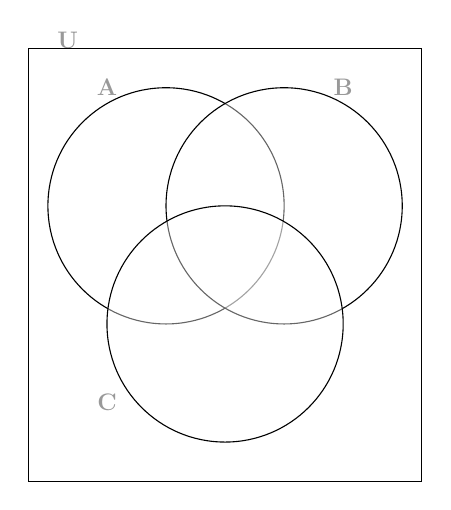
\begin{tikzpicture}[scale=0.5, transform shape]
    %% You can adjust the opacity here. For venn diagrams it is convenient to have a low opacity so that you can see intersections
        \begin{scope} [fill opacity = 0.4]
    %% The draw command knows a lot of shapes. To make a rectangle you just need to specify two diagonal corners. Make sure you always have a semicolon at the end of your draw commands, otherwise latex flips out.
        \draw (-5,5) rectangle (5,-6);
    %% Similarly, you can make a circle by specifying the center and then the radius. You can also add a fill color, but if you're printing in black and white you'll probably want to remove that line.
        \draw[fill=white, draw = black] (-1.5,1) circle (3);
        \draw[fill=white, draw = black] (1.5,1) circle (3);
        \draw[fill=white, draw = black] (0,-2) circle (3);
    %% We can use the node command to label points. If you put your cursor on "LARGE" or "textbf" a box will drop down with size and text style options.
        \node at (-4,5.2) {\LARGE\textbf{U}};
        \node at (-3,4) {\LARGE\textbf{A}};
        \node at (3,4) {\LARGE\textbf{B}};
        \node at (-3,-4) {\LARGE\textbf{C}};
        \end{scope}
    %% And now you have a venn diagram. Yay!
    %\draw[help lines](-5,5) grid (5,-6);    This line can draw the grid lines to help guide you. I use these when I'm writing the code and then delete this line when I publish the pdf.
\end{tikzpicture}

\subsection*{ii. \( (A \cup B) - C \)}

%% This block is what you'll need to put in your code where you want your picture.
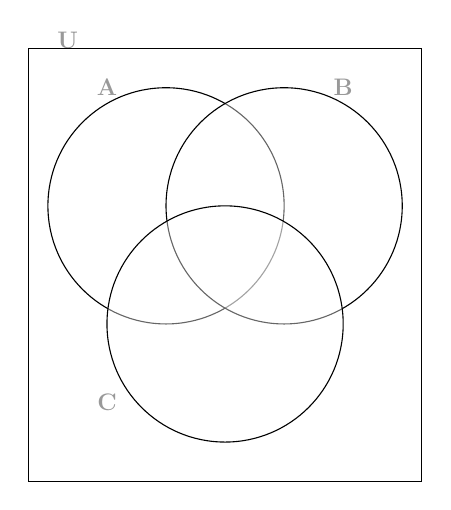
\begin{tikzpicture}[scale=0.5, transform shape]
    %% You can adjust the opacity here. For venn diagrams it is convenient to have a low opacity so that you can see intersections
        \begin{scope} [fill opacity = 0.4]
    %% The draw command knows a lot of shapes. To make a rectangle you just need to specify two diagonal corners. Make sure you always have a semicolon at the end of your draw commands, otherwise latex flips out.
        \draw (-5,5) rectangle (5,-6);
    %% Similarly, you can make a circle by specifying the center and then the radius. You can also add a fill color, but if you're printing in black and white you'll probably want to remove that line.
        \draw[fill=white, draw = black] (-1.5,1) circle (3);
        \draw[fill=white, draw = black] (1.5,1) circle (3);
        \draw[fill=white, draw = black] (0,-2) circle (3);
    %% We can use the node command to label points. If you put your cursor on "LARGE" or "textbf" a box will drop down with size and text style options.
        \node at (-4,5.2) {\LARGE\textbf{U}};
        \node at (-3,4) {\LARGE\textbf{A}};
        \node at (3,4) {\LARGE\textbf{B}};
        \node at (-3,-4) {\LARGE\textbf{C}};
        \end{scope}
    %% And now you have a venn diagram. Yay!
    %\draw[help lines](-5,5) grid (5,-6);    This line can draw the grid lines to help guide you. I use these when I'm writing the code and then delete this line when I publish the pdf.
\end{tikzpicture}

\subsection*{iii. \( A^C \cap B^C \)}

%% This block is what you'll need to put in your code where you want your picture.
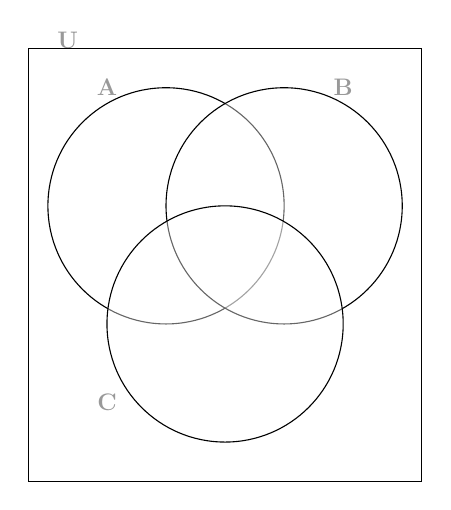
\begin{tikzpicture}[scale=0.5, transform shape]
    %% You can adjust the opacity here. For venn diagrams it is convenient to have a low opacity so that you can see intersections
        \begin{scope} [fill opacity = 0.4]
    %% The draw command knows a lot of shapes. To make a rectangle you just need to specify two diagonal corners. Make sure you always have a semicolon at the end of your draw commands, otherwise latex flips out.
        \draw (-5,5) rectangle (5,-6);
    %% Similarly, you can make a circle by specifying the center and then the radius. You can also add a fill color, but if you're printing in black and white you'll probably want to remove that line.
        \draw[fill=white, draw = black] (-1.5,1) circle (3);
        \draw[fill=white, draw = black] (1.5,1) circle (3);
        \draw[fill=white, draw = black] (0,-2) circle (3);
    %% We can use the node command to label points. If you put your cursor on "LARGE" or "textbf" a box will drop down with size and text style options.
        \node at (-4,5.2) {\LARGE\textbf{U}};
        \node at (-3,4) {\LARGE\textbf{A}};
        \node at (3,4) {\LARGE\textbf{B}};
        \node at (-3,-4) {\LARGE\textbf{C}};
        \end{scope}
    %% And now you have a venn diagram. Yay!
    %\draw[help lines](-5,5) grid (5,-6);    This line can draw the grid lines to help guide you. I use these when I'm writing the code and then delete this line when I publish the pdf.
\end{tikzpicture}

\subsection*{iv. \( ((A^C \cup B^C) \cup C^C)^C \)}

%% This block is what you'll need to put in your code where you want your picture.
%% This block is what you'll need to put in your code where you want your picture.
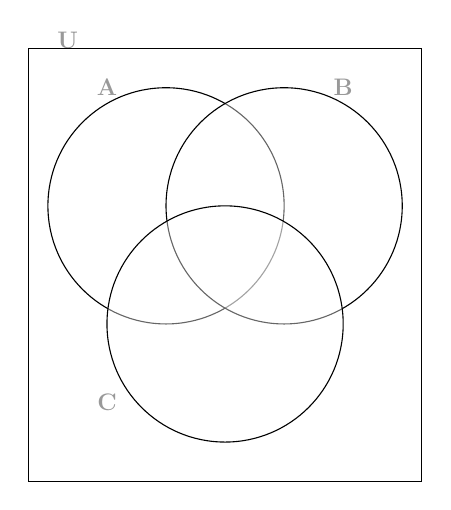
\begin{tikzpicture}[scale=0.5, transform shape]
    %% You can adjust the opacity here. For venn diagrams it is convenient to have a low opacity so that you can see intersections
        \begin{scope} [fill opacity = 0.4]
    %% The draw command knows a lot of shapes. To make a rectangle you just need to specify two diagonal corners. Make sure you always have a semicolon at the end of your draw commands, otherwise latex flips out.
        \draw (-5,5) rectangle (5,-6);
    %% Similarly, you can make a circle by specifying the center and then the radius. You can also add a fill color, but if you're printing in black and white you'll probably want to remove that line.
        \draw[fill=white, draw = black] (-1.5,1) circle (3);
        \draw[fill=white, draw = black] (1.5,1) circle (3);
        \draw[fill=white, draw = black] (0,-2) circle (3);
    %% We can use the node command to label points. If you put your cursor on "LARGE" or "textbf" a box will drop down with size and text style options.
        \node at (-4,5.2) {\LARGE\textbf{U}};
        \node at (-3,4) {\LARGE\textbf{A}};
        \node at (3,4) {\LARGE\textbf{B}};
        \node at (-3,-4) {\LARGE\textbf{C}};
        \end{scope}
    %% And now you have a venn diagram. Yay!
    %\draw[help lines](-5,5) grid (5,-6);    This line can draw the grid lines to help guide you. I use these when I'm writing the code and then delete this line when I publish the pdf.
\end{tikzpicture}

\subsection*{v. \( (B^C \cap B) \cup (C \cap A) \)}

%% This block is what you'll need to put in your code where you want your picture.
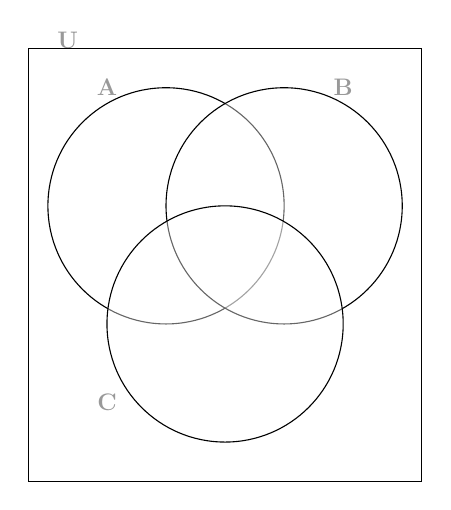
\begin{tikzpicture}[scale=0.5, transform shape]
    %% You can adjust the opacity here. For venn diagrams it is convenient to have a low opacity so that you can see intersections
        \begin{scope} [fill opacity = 0.4]
    %% The draw command knows a lot of shapes. To make a rectangle you just need to specify two diagonal corners. Make sure you always have a semicolon at the end of your draw commands, otherwise latex flips out.
        \draw (-5,5) rectangle (5,-6);
    %% Similarly, you can make a circle by specifying the center and then the radius. You can also add a fill color, but if you're printing in black and white you'll probably want to remove that line.
        \draw[fill=white, draw = black] (-1.5,1) circle (3);
        \draw[fill=white, draw = black] (1.5,1) circle (3);
        \draw[fill=white, draw = black] (0,-2) circle (3);
    %% We can use the node command to label points. If you put your cursor on "LARGE" or "textbf" a box will drop down with size and text style options.
        \node at (-4,5.2) {\LARGE\textbf{U}};
        \node at (-3,4) {\LARGE\textbf{A}};
        \node at (3,4) {\LARGE\textbf{B}};
        \node at (-3,-4) {\LARGE\textbf{C}};
        \end{scope}
    %% And now you have a venn diagram. Yay!
    %\draw[help lines](-5,5) grid (5,-6);    This line can draw the grid lines to help guide you. I use these when I'm writing the code and then delete this line when I publish the pdf.
\end{tikzpicture}

\subsection*{vi. \( (C - A) \cup (A - B) \cup (B - C) \)}

%% This block is what you'll need to put in your code where you want your picture.
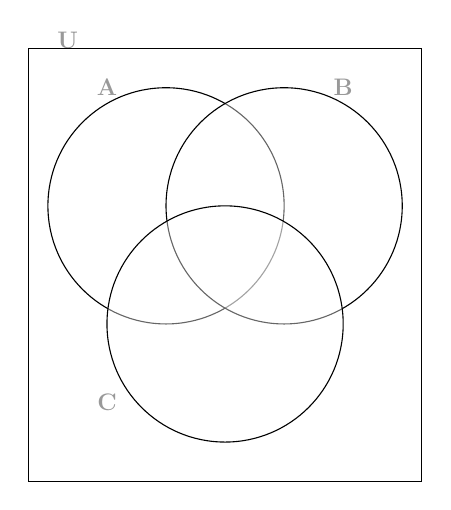
\begin{tikzpicture}[scale=0.5, transform shape]
    %% You can adjust the opacity here. For venn diagrams it is convenient to have a low opacity so that you can see intersections
        \begin{scope} [fill opacity = 0.4]
    %% The draw command knows a lot of shapes. To make a rectangle you just need to specify two diagonal corners. Make sure you always have a semicolon at the end of your draw commands, otherwise latex flips out.
        \draw (-5,5) rectangle (5,-6);
    %% Similarly, you can make a circle by specifying the center and then the radius. You can also add a fill color, but if you're printing in black and white you'll probably want to remove that line.
        \draw[fill=white, draw = black] (-1.5,1) circle (3);
        \draw[fill=white, draw = black] (1.5,1) circle (3);
        \draw[fill=white, draw = black] (0,-2) circle (3);
    %% We can use the node command to label points. If you put your cursor on "LARGE" or "textbf" a box will drop down with size and text style options.
        \node at (-4,5.2) {\LARGE\textbf{U}};
        \node at (-3,4) {\LARGE\textbf{A}};
        \node at (3,4) {\LARGE\textbf{B}};
        \node at (-3,-4) {\LARGE\textbf{C}};
        \end{scope}
    %% And now you have a venn diagram. Yay!
    %\draw[help lines](-5,5) grid (5,-6);    This line can draw the grid lines to help guide you. I use these when I'm writing the code and then delete this line when I publish the pdf.
\end{tikzpicture}

\newpage

\section*{Problem 4: Set Algebra}

\subsection*{i. \( A \cap A \)}
Using the Idempotent Law:
\[
A \cap A = A
\]

\subsection*{ii. \( (A^C \cap B^C)^C \cap U \)}
Applying De Morgan's Law and simplifying:
\[
(A^C \cap B^C)^C = A \cup B, \quad A \cup B \cap U = A \cup B
\]
Answer: \( A \cup B \)

\subsection*{iii. \( (A \cup A) \cap (B \cup A^C) \)}
Using the Idempotent Law and simplifying:
\[
A \cup A = A, \quad B \cup A^C = U, \quad A \cap U = A
\]
Answer: \( A \)

\newpage

\section*{Problem 5: Set Builder Notation}

\subsection*{i. Set \(S = \{n \in \mathbb{Z} \mid n \in \mathbb{N} \text{ and } -5 \leq n < 7\} \)}
Listing the elements:
\[
S = \{0, 1, 2, 3, 4, 5, 6\}
\]

\subsection*{ii. Express the set \(B\) of integers whose fourth power is either 16 or 81.}
Using set-builder notation:
\[
B = \{x \in \mathbb{Z} \mid x^4 = 16 \text{ or } x^4 = 81\}
\]

\subsection*{iii. Listing the elements of \(B\):}
\[
B = \{-3, -2, 2, 3\}
\]

\newpage

\section*{Problem 6: Digital Circuit}

\subsection*{i. Expression for \(Y\) in terms of \(A\), \(B\), and \(C\):}
From the circuit:
\[
Y = \neg((A \land B) \lor \neg C)
\]

\subsection*{ii. Simplifying \(Y\) using logic identities:}
First, apply Demorgan's Law:
\[
Y = \neg(A \land B) \and \neg C
\]
Second, apply involution:
\[
Y = \neg (A \land B) \land C
\]
Third, apply De Morgan's Law:
\[
Y = (\neg A \lor \neg B) \land C
\]

\subsection*{iii. Drawing the circuit:}

\begin{figure}[!ht]
    \centering
    \resizebox{1\textwidth}{!}{%
    \begin{circuitikz}
    \tikzstyle{every node}=[font=\LARGE]
    \node [font=\LARGE] at (5.25,13) {};
    \draw (6.75,13) to[short] (8.25,13);
    \draw (8.5,13) node[ieeestd not port, anchor=in](port){} (port.out) to[short] (10.25,13);
    \draw (port.in) to[short] (8.25,13);
    \node [font=\LARGE] at (6.5,13) {A};
    \draw (6.75,11.5) to[short] (8.25,11.5);
    \node [font=\LARGE] at (6.5,11.5) {B};
    \draw (8.5,11.5) node[ieeestd not port, anchor=in](port){} (port.out) to[short] (10.25,11.5);
    \draw (port.in) to[short] (8.25,11.5);
    \draw (12.75,12.25) to[short] (13,12.25);
    \draw (12.75,11.75) to[short] (13,11.75);
    \draw (13,12.25) node[ieeestd and port, anchor=in 1, scale=0.89](port){} (port.out) to[short] (14.75,12);
    \draw (10.25,11.5) to[short] (10.75,12);
    \draw (10.25,13) to[short] (10.75,12.5);
    \draw (10.75,12.5) to[short] (11,12.5);
    \draw (10.75,12) to[short] (11,12);
    \draw (11,12.5) node[ieeestd or port, anchor=in 1, scale=0.89](port){} (port.out) to[short] (12.75,12.25);
    \draw [short] (10.75,10.25) -- (12.75,11.75);
    \draw [short] (6.75,10.25) -- (10.75,10.25);
    \node [font=\LARGE] at (6.5,10.5) {};
    \node [font=\LARGE] at (6.5,10.5) {};
    \node [font=\LARGE] at (15,12) {};
    \node [font=\LARGE] at (15,12) {};
    \node [font=\LARGE] at (15,12) {Y};
    \node [font=\LARGE] at (6.5,10.5) {};
    \node [font=\LARGE] at (6.5,10.5) {};
    \node [font=\LARGE] at (6.5,10.5) {};
    \node [font=\LARGE] at (6.5,10.5) {};
    \node [font=\LARGE] at (6.5,10.5) {};
    \node [font=\LARGE] at (6.5,10.25) {C};
    \end{circuitikz}
    }%
    
    \label{fig:my_label}
    \end{figure}
\end{document}
